
\section{Security of third party apps}

\subsection{App runtime}

The applications are intended to be run on a wide range of devices, with different hardware configurations.
The execution environment needs to be able to enforce access control and isolation.
Moreover, the devices are very limited in resources, which makes it difficult to adapt the existing solutions such as Java virtual machine.
For those reasons, Garmin decided to create a custom virtual machine and a programming language.

However, creating a correct abstraction layer is a complex task.
It creates a large attack surface, and it is challenging to ensure that the implementation is correct.

\subsection{Preliminary analysis}
The existing research analysed the bytecode of the firmware running on the watch.
Unfortunately, the firmware is no longer available for download.
There is a chance that it would be possible to reverse engineer the watch hardware and extract the firmware from the device.
However, it would require an extensive amount of time and resources and is out of scope of this report.
Another option would be to investigate the protocol used to download a new firmware version.
It would require additional time and there is no guarantee that it would be possible to download the full firmware.

In the end, I decided to perform the analysis on the simulator provided by Garmin.
As it runs directly on the computer, it is possible to perform a more in-depth analysis of the software such as dynamic analysis.
The simulator is supposed to guarantee proper isolation, so escaping the sandbox would be a potential vulnerability.
Additionally, there is a chance that parts of the code are reused in the firmware running on the watch and the findings would be applicable to the real device.

\subsection{Permissions}

Third party apps can interact with the watch by using the API provided by the SDK.
The API is divided into several modules, each of them providing different functionality.
Some of those functionalities can be considered sensitive, such as GPS location, heart rate, or access to the internet.
Because of that, Garmin implemented a permission system, where different permissions grant access to different modules.
The app has to define in the manifest file which permissions it requires, and the user has to accept them before installing the app.
The system offers some granularity, and can give the user a general overview of what the app can do.
However, some, potentially sensitive modules don't require any permissions.
For example, the app can access some basic activity data such as heart rate, steps, calories without any permissions.
Moreover, in February 2023, Garmin introduced a new module: Complications.
It is a publish/subscribe model that allows for the apps to publish different metrics, so that they would be accessible for any watch face.
While it makes the access to different metrics more flexible and accessible, it also removes the granularity of the permissions.
Every app can potentially publish very sensitive data, without the user being aware of it.
Then every watch face can access all this data if it requests `Complications` permission.

\subsection{Building process}
In order to understand the runtime environment, I started with the analysis of the building process.

During the compilation, the code is translated to mid-level intermediate representation (MIR).
The files containing the representations are created during the build process and could be used for better understanding of the final artifact.

The compiler is written in Java, which makes the analysis of the code relatively simple.
Nonetheless, the compilation is a complicated process consisting of several stages.

For the analysis, I decided to use JADX decompiler\cite{jadx}.
After loading the jar file, I noticed that a large part of the important code is not obfuscated.


Java class `Opcode` contains a list of instructions in the final bytecode.
Additionally, SDK provides a mapping of all API methods to the number values, which is probably some type of address.

I was able to find the code responsible for signing the application.
It is describe in more detail in the section~\ref{subsec:signing}.

\subsection{Bytecode analysis}

\subsection{Simulator}
Garmin SDK provides a simulator for testing the apps.
It is used by the Visual Studio Code extension to run the apps.
I found the executable in the SDK bin folder.
The file starts with ELF header, which means that it is a binary executable file.
To analyse bytecode, I decided to use Ghidra\cite{ghidra}.
It is free and open-source software for reverse engineering.

After loading the file, a list of assembly instructions is displayed.
Fortunately, Ghidra has an option to analyse and decompile the code to C\@.

\begin{figure}[h]
    \centering
    \includegraphics[width=1\linewidth]{../../images/ghidra2}
    \caption{Simulator decompilation}
    \label{fig:concept}
\end{figure}

The header of the third party apps is tagged with value `0xD000D000`\cite{broken-vm}.
Searching for it in the simulator binary reveals two references.

From this point, it would be theoretically possible to analyse the code and reverse engineer the virtual machine.
However, doing it without any documentation, where the names of the functions and variables are not known would be very challenging.
As it is not possible to do it in a reasonable amount of time, I decided to focus on fuzzing the virtual machine.
This is described in the section~\ref{sec:fuzzing}.

\subsection{Modifying the executable}
In order to test the security of the virtual machine, it is useful to be able to edit the executable.
However, after changing the bytecode, it is necessary to sign the executable again.
After analysis of \textit{monkeybrains.jar} file, I created a kotlin script that signs the app again.
\subsection{Signing} \label{subsec:signing}
The generated app bytecode has to be signed by the developer.
The signing algorithm uses SHA1 hash of the bytecode that is signed with a private RSA key.
The key is 4096 long, which is more than recommended.

For the signing, conventions described in PKCS \#1 v2.2 are used.

SHA-1 is no longer considered secure against well-funded opponents.
NIST formally deprecated use of this hash function in 2011.
In 2020 there was a paper published demonstrating a chosen-prefix collision attack.
It still doesn't offer a viable solution to find a collision to a given hash for a chosen prefix.
However, the function has been already broken and in the upcoming years new attacks might be discovered.

Algorithm for signing:
- read bytes from PRG file that hasn't been signed yet
- don't include the bytes at the end of the file (called TERMINATOR in the code)
- compute the signature with Java security signature library (SHA1withRSA)
- Append the file bytes Developer signature, consisting of:
- magic number
- length of the whole signature
- signature
- modulus
- exponent
- Or in the case of the store signature:
- a different magic number
- length of the whole signature
- signature
- Append the terminating bytes that were skipped before

\subsection{Communication between the watch and the phone} \label{subsec:communication-watch-phone}

Garmin apps define their own permissions.
One of them is for example \verb|com.garmin.android.apps.connectmobile.permission.RECEIVE_BROADCASTS|, which allows to listen for action \verb|ACTION_ON_FIND_MY_PHONE_MESSAGE_RECEIVED|, which triggers sound on the phone.
I don't know, however, who sends this action.

\textbf{Privacy issue 1} - Every app can register for garmin ConnectIQ service without registering any permissions.
It can give the information if and what Garmin device the user has connected to the phone.

It seems like any phone app can receive events from all watch apps.
There is no authentication.

I have a proof of concept, but idk which apps are using it, if any\ldots

According to Android documentation: [About broadcasts](https://developer.android.com/guide/components/broadcasts),
it is possible to send broadcasts that can be only received by apps with specific permissions.
It is also possible to define a custom permission.
However, custom permissions have to be already defined when such app is being installed.
Because of that, it is probably not a viable option for Garmin.

%\begin{figure}[h]
%    \centering
%    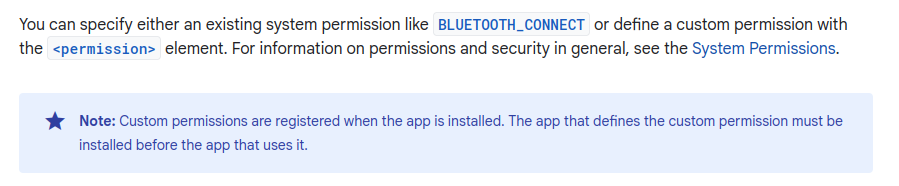
\includegraphics[width=1\linewidth]{images/android-custom-permissions-note.png}
%    \caption{Android custom permissions note}
%    \label{fig:concept}
%\end{figure}

\subsection{Sandboxing}